\documentclass[12pt]{article}

\usepackage{geometry}
\geometry{letterpaper}
\geometry{margin=1in}
\linespread{1.1}
\renewcommand{\familydefault}{\sfdefault}
\raggedright

\usepackage[
	style=ieee,
]{biblatex}
\addbibresource{conceptproposal.bib}

\usepackage{booktabs} % for much better looking tables
\usepackage{array} % for better arrays (eg matrices) in maths
\usepackage{paralist} % very flexible & customisable lists (eg. enumerate/itemize, etc.)
\usepackage{verbatim} % adds environment for commenting out blocks of text & for better verbatim
\usepackage{subfigure} % make it possible to include more than one captioned figure/table in a single float
\usepackage{graphicx}
\usepackage[rightcaption]{sidecap}

\usepackage{amsfonts}
\usepackage{amssymb}
\usepackage{relsize}
\usepackage{tikz}
\usetikzlibrary{matrix,fit,calc}

\newcounter{enumine}

\title{STRATODUSTER\\Concept Proposal}
\author{Jimmy Vaughan\\101 156 687\\Group 57 (solo)}
\date{February 16, 2024}

%%% BEGIN DOCUMENT
\begin{document}

\maketitle
\thispagestyle{empty}
\setcounter{tocdepth}{2}
\vfill
\tableofcontents
\clearpage

~
\vfill
\listoffigures
\listoftables
\clearpage

\pagestyle{headings}

\section{Introduction}
\subsection{Purpose}
The purpose of this project is to design an aircraft capable of performing Stratospheric Aerosol Injection (SAI) \cite{Smith:2018aa} of liquid sulfuric acid or another liquid aerosol.
This mission is part of an extreme potential measure that can be undertaken quickly by world powers, should an acute need arise for planetary cooling.
By dispensing aerosol into the air at high altitude to reflect some solar radiation, the planetary energy balance can be adjusted to reduce temperatures \cite{Bradley:2023aa}.


\subsection{Mission Requirements}
There are two missions specified in the request for proposal (RFP): a Payload Dispensing Mission (PDM) and a Ferry Mission (FM). 
Considerations for the PDM are: the payload weight changes over the course of the cruise legs, dropping to zero at the end of the second; payload is a liquid, so its movement will affect centre of gravity.
The main consideration for the FM is the range.

The key general requirements are:
\begin{compactenum}
	\item Cruise Mach over 0.5
	\item Capable of flight in known icing conditions
	\item Certifiable to FAA 14 CFR Part 25 Standards
	\item Flight crew of 4, no passengers
	\item Time to climb of less than 1 hour
\setcounter{enumine}{\value{enumi}}
\end{compactenum}

The mission requirements are, for the Payload Dispensing Mission:
\begin{compactenum}
\setcounter{enumi}{\value{enumine}}
	\item Minimum payload weight of 30,000 lb
	\item Payload density of 15 lb/gal
	\item Cruise range of 400 nmi round-trip, loaded
\setcounter{enumine}{\value{enumi}}
\end{compactenum}

And for the Ferry Mission:
\begin{compactenum}
\setcounter{enumi}{\value{enumine}}
	\item Minimum range of 3,000 nmi, unloaded
\setcounter{enumine}{\value{enumi}}
\end{compactenum}

And for both missions,
\begin{compactenum}
\setcounter{enumi}{\value{enumine}}
	\item Maximum takeoff and landing field lengths of 8,000' over a 50' obstacle
	\item Capable of taking off and landing from (dry) concrete runways
	\item Capable of VFR and IFR flight
\end{compactenum}

Other considerations are the systems and components needed to fly in both controlled and uncontrolled airspaces, and an entry into service (EIS) date of 2030.
The RFP also asks for a fleet size capable of dispensing 3 million metric tons of payload per year, when flown daily.
The main objective is to minimize the total cost of building and operating the aircraft per mass of payload dispensed \cite{Bradley:2023aa}.


\subsection{Existing Aircraft}
The performance of three representative aircraft that have similar mission capabilities to those prescribed in the previous section is summarized in brief in Table~\ref{tab:exist}.
\begin{table}[h]
	\centering
	\begin{tabular}{@{}lcccccc@{}}
		\toprule
		Aircraft & Gross Weight & Cruise Speed & Service Ceiling & Range & Payload & Thrust \\
		\midrule
		Global 8000 & 105,000 lb & Mach 0.90 & 51,000 ft & 5,650 nmi & 5,700 lb & 33,000 lbf \\
		B-52H & 488,000 lb & Mach 0.84 & 50,000 ft & 7,600 nmi & 70,000 lb & 136,000 lbf \\
		Falcon 8X & 73,000 lb & Mach 0.90 & 51,000 ft & 6,450 nmi & 4,900 lb & 20,175 lbf \\
		\bottomrule
	\end{tabular}
	\caption{Performance of Representative High-Altitude Aircraft~\cite{Janes:2023ab}~\cite{Force:2019aa}~\cite{Janes:2023aa}}
	\label{tab:exist}
\end{table}

It's been challenging finding aircraft that match the mission requirements closely.
Most aircraft that are capable of stratospheric flight are specialized or supersonic aircraft designed for various military applications.
Some are ultralights, powered by solar arrays, or lighter-then-air aircraft, and are designed for classified purposes or imaging/communications~\cite{Piesing:2023aa}.
The choices presented here are all long-range aircraft.
The hope is that minimal modification would be needed to their configurations to increase the service ceiling and payload capacity by reducing range.


\subsubsection{Bombardier Global 8000}
\begin{SCfigure}[0.66][h]
	\centering
	\includegraphics[width=0.4\textwidth]{Global8000}
	\caption{A Bombardier Global 8000 Aircraft~\cite{pic:G8000}}
	\label{fig:G8000}
\end{SCfigure}

The Bombardier~Global~8000, shown in Figure~\ref{fig:G8000}, is a long-range business jet aircraft with rear-mounted GE turbofan engines.
It's an extension of the Global~6000, but has transonic wings with increased area and reduced thickness, as well as redesigned winglets.
The Global 8000 is certified for between eight and seventeen passengers, making it a GA aircraft.
The closely related Global~7500 broke several range and speed records in 2019, flying over 8,225~nmi from Sydney to Detroit, among other accomplishments~\cite{Janes:2023ab}.

The listed payload is under what is required by the mission requirements, but the general characteristics of the plane are quite attractive.
It flies close to the speed of sound, and has a high service ceiling with a very long range.
With modifications to the configuration, it could provide a good base for a cargo/dispensing mission slightly higher in the stratosphere.


\subsubsection{Boeing B-52 Stratofortress}
\begin{SCfigure}[0.7][h]
	\centering
	\includegraphics[width=0.4\textwidth]{B-52H}
	\caption{A Boeing B-52H Stratofortress in flight over the Persian Gulf~\cite{pic:B52H}}
	\label{fig:B52H}
\end{SCfigure}

The Boeing~B-52~Stratofortress, shown in Figure~\ref{fig:B52H} as a B-52H, is a long-range heavy bomber that has been in service for over 60 years, and is expected to remain in use until the 2050s.
It is capable of flying at high subsonic speeds at high altitudes, and has an incredible range of 8,800~nmi without refueling.
With the ability to carry approximately 70,000~lb of weapons payload, and boasting eight turbofan engines, the B-52H is a formidable heavy bomber~\cite{Force:2019aa}.

It is, of course, overkill for a mission that requires only half the payload and less than a tenth of the range, but it is proof that heavy cargo is possible at high altitude.
The success of the B-52 platform is indication that high-altitude aircraft are a worthwhile investment.


\subsubsection{Dassault Falcon 8X}
\begin{SCfigure}[0.8][h]
	\centering
	\includegraphics[width=0.4\textwidth]{F8X}
	\caption{Dassault Falcon 8X at Paris Air Show 2019~\cite{pic:F8X}}
	\label{fig:F8X}
\end{SCfigure}

The Dassault~Falcon~8X, shown in Figure~\ref{fig:F8X}, is a long-range business tri-jet with the longest cabin in the Falcon family.
Not only is it used for business aviation, but a special missions version is also being developed for the French~Armed~Forces, known as Archange.
The Falcon~8X's improvements over the 7X are improved engines, revised wing design, and lighter construction~\cite{Janes:2023aa}.

The tri-jet design may pose a challenge, if the sulfuric acid aerosol is to be dispensed from the wings (in front of the jet intakes).
The long range and fast cruising speed are both advantages, as well as the general versatility of the design.
The Falcon~8X comes from a family of high-performance aircraft, and boasts desirable improvements over its predecessors.


\section{Concept Selection}
\subsection{QFD Analysis}

\begin{figure}[h!]
\centering
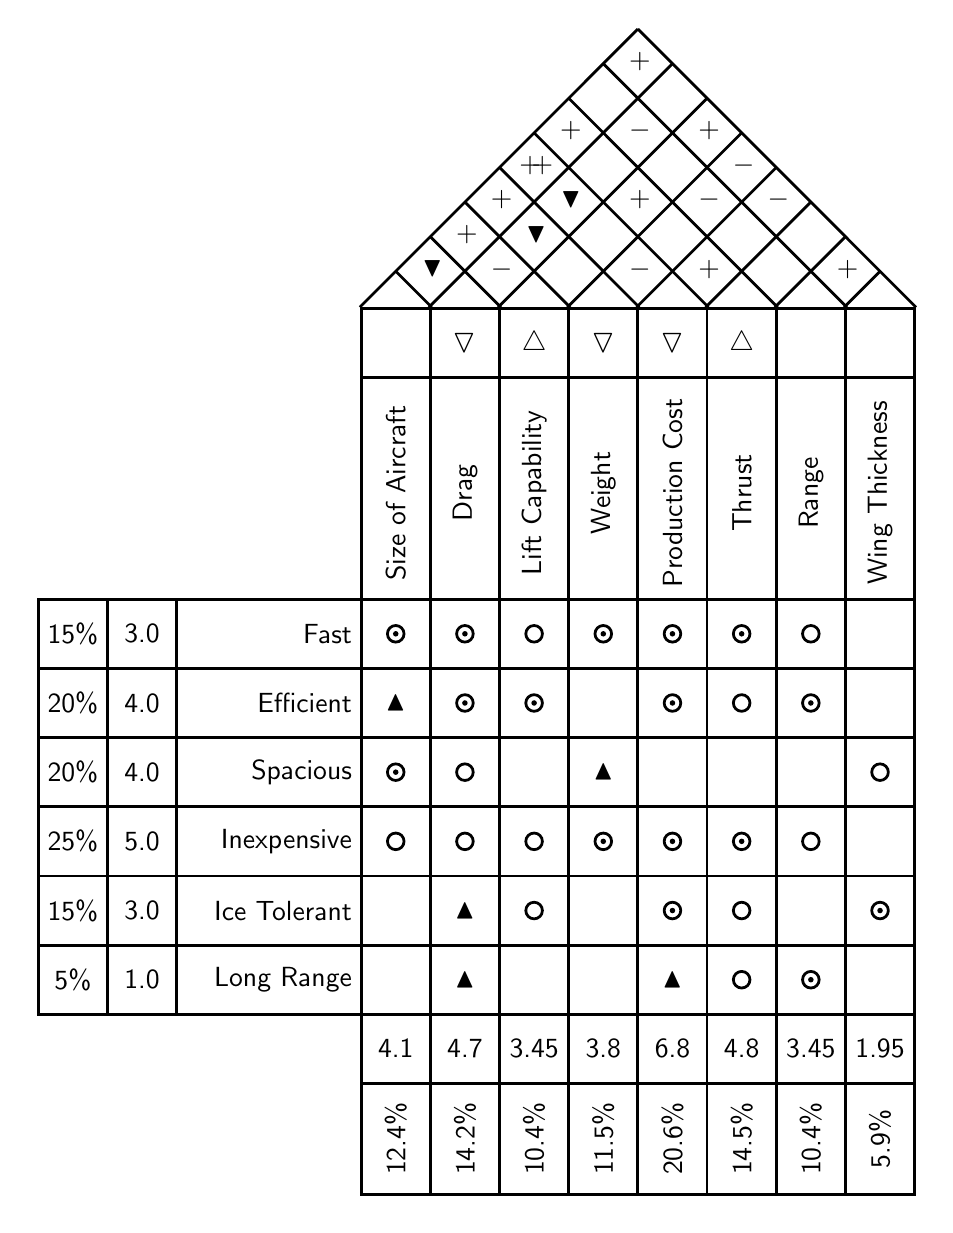
\begin{tikzpicture}[font=\sffamily,myfit/.style={fill=white,draw,line width=\mylinewidth,
 inner sep=-0.5*\mylinewidth,fit=#1},
 circ/.style={path picture={\draw circle (0.3em);}},
 circdot/.style={path picture={\draw circle (0.3em); 
 \fill circle (0.1em);}},
 trian/.style={path picture={\draw (-30:0.3em) -- (90:0.3em) -- (210:0.3em) --cycle ;}},
 ]
 \def\mylinewidth{1pt}
 \def\hw{2.5em}
 \matrix[matrix of nodes, nodes={draw,line width=\mylinewidth,minimum width=\hw,
 minimum height=\hw, anchor=center},column sep=-\mylinewidth,
 ,row sep=-\mylinewidth,%nodes in empty cells,
 row 2/.style={nodes={align=left,rotate=90,minimum width=8em,minimum height=\hw}},
 row 10/.style={nodes={rotate=90,minimum width=4em,minimum height=\hw}},
 column 3/.style={nodes={align=right,text width=6em,}}](mat) {
    %& & & ~ & ~& ~ & ~& ~& ~& ~&~ \\
    & & & ~ & \large$\triangledown$ & $\triangle$ & \large$\triangledown$ & \large$\triangledown$ & $\triangle$ & ~ &~ \\
    & & & Size of Aircraft & Drag & Lift Capability & Weight & Production Cost & Thrust & Range & Wing Thickness \\
   15\%& 3.0& Fast & |[circdot]| & |[circdot]| & |[circ]| & |[circdot]| & |[circdot]| & |[circdot]| & |[circ]| &~ \\
   20\%& 4.0& Efficient & $\blacktriangle$ & |[circdot]| & |[circdot]|  & ~& |[circdot]|& |[circ]|& |[circdot]|&~ \\
   20\%& 4.0& Spacious & |[circdot]|  & |[circ]| & ~ & $\blacktriangle$ & ~& ~& ~&|[circ]| \\
   25\%& 5.0& Inexpensive & |[circ]|  & |[circ]|& |[circ]| & |[circdot]| &|[circdot]|& |[circdot]|& |[circ]|&~ \\
   15\%& 3.0& Ice Tolerant &  ~ & $\blacktriangle$& |[circ]| & ~& |[circdot]| & |[circ]| & ~&|[circdot]| \\
   5\%& 1.0& Long Range &  ~ & $\blacktriangle$ & ~ & ~& $\blacktriangle$& |[circ]|& |[circdot]|&~ \\
    & & & 4.1 & 4.7 & 3.45 & 3.8 & 6.8 & 4.8 & 3.45 &1.95  \\
    & & & 12.4\% & 14.2\% & 10.4\% & 11.5\% & 20.6\% & 14.5\% & 10.4\% & 5.9\% \\
 };
 %\node[myfit=(mat-1-4) (mat-1-11)] {thermometre};
 %\node[myfit=(mat-2-4) (mat-2-7)] {capteur};
 %\node[myfit=(mat-2-8) (mat-2-9)] {etal};
 %\node[myfit=(mat-8-1) (mat-3-1)] (aux1){};
 %\node[rotate=90] at (aux1){Customer Requirements};
 %\node[myfit=(mat-6-2) (mat-4-2)] (aux2){};
 %\node[rotate=90] at (aux2){Payload};
 %\node[rotate=90] at (mat-9-2) {};
 % etc.
 \foreach \X in {4,...,11}
 {\draw[line width=\mylinewidth] (mat-1-\X.north west)
 -- (intersection cs:first line={(mat-1-\X.north west)--($(mat-1-\X.north west)+(45:5)$)},
 second line={(mat-1-11.north east)--($(mat-1-11.north east)+(135:5)$)});
 \draw[line width=\mylinewidth] (mat-1-\X.north east)
 -- (intersection cs:first line={(mat-1-\X.north east)--($(mat-1-\X.north east)+(135:5)$)},
 second line={(mat-1-4.north west)--($(mat-1-4.north west)+(45:5)$)});
 }
 \begin{scope}[shift={(mat-1-4.north west)},
 x={(45:{sqrt(1/2)*\hw})},y={(-45:{sqrt(1/2)*\hw})}
 ] % define local coordinate system for easier access of the cells
 \begin{scope}[shift={(0.6,-0.5)}]
  \foreach \Coord in {(2,1),(3,1),(5,1),%
  (7,1),(5,3),(7,3),(5,5),(7,7)}
  {\node at \Coord {+};}
  \foreach \Coord in {(4,1)}{\node at \Coord {$\mathbin{+\mkern-6mu+}$};}
  \foreach \Coord in {(1,1),(3,2),(4,2)}{\node at \Coord {$\blacktriangledown$};}
  \foreach \Coord in {(2,2),(6,2),(4,4),(6,4),(7,4),(7,5)}{\node at \Coord {$-$};}
 \end{scope} 
 \end{scope}
\end{tikzpicture}
\caption{Quality Function Deployment Matrix (House of Quality) for STRATODUSTER.}
\label{fig:hq}
\end{figure}

The house of quality matrix in Figure~\ref{fig:hq}, produced with much modification and effort from~\cite{user121799:2019aa}, provides insights into which engineering challenges command the most focus.
As stated in the RFP, the primary goal of the mission is to minimize the cost of payload delivery~\cite{Bradley:2023aa}, which will be primarily through minimizing production cost, and secondarily minimizing operating costs, where possible.
There aren't that many explicit customer requirements in the RFP, besides functional ones, but the fact that it's a government based RFP indicates that they have a high priority on value, or at least, efficient use of resources.
In other words, inexpensive and long-lasting.
% TODO: more?

\subsection{General Configuration}
\begin{SCfigure}[0.2][h]
	\centering
	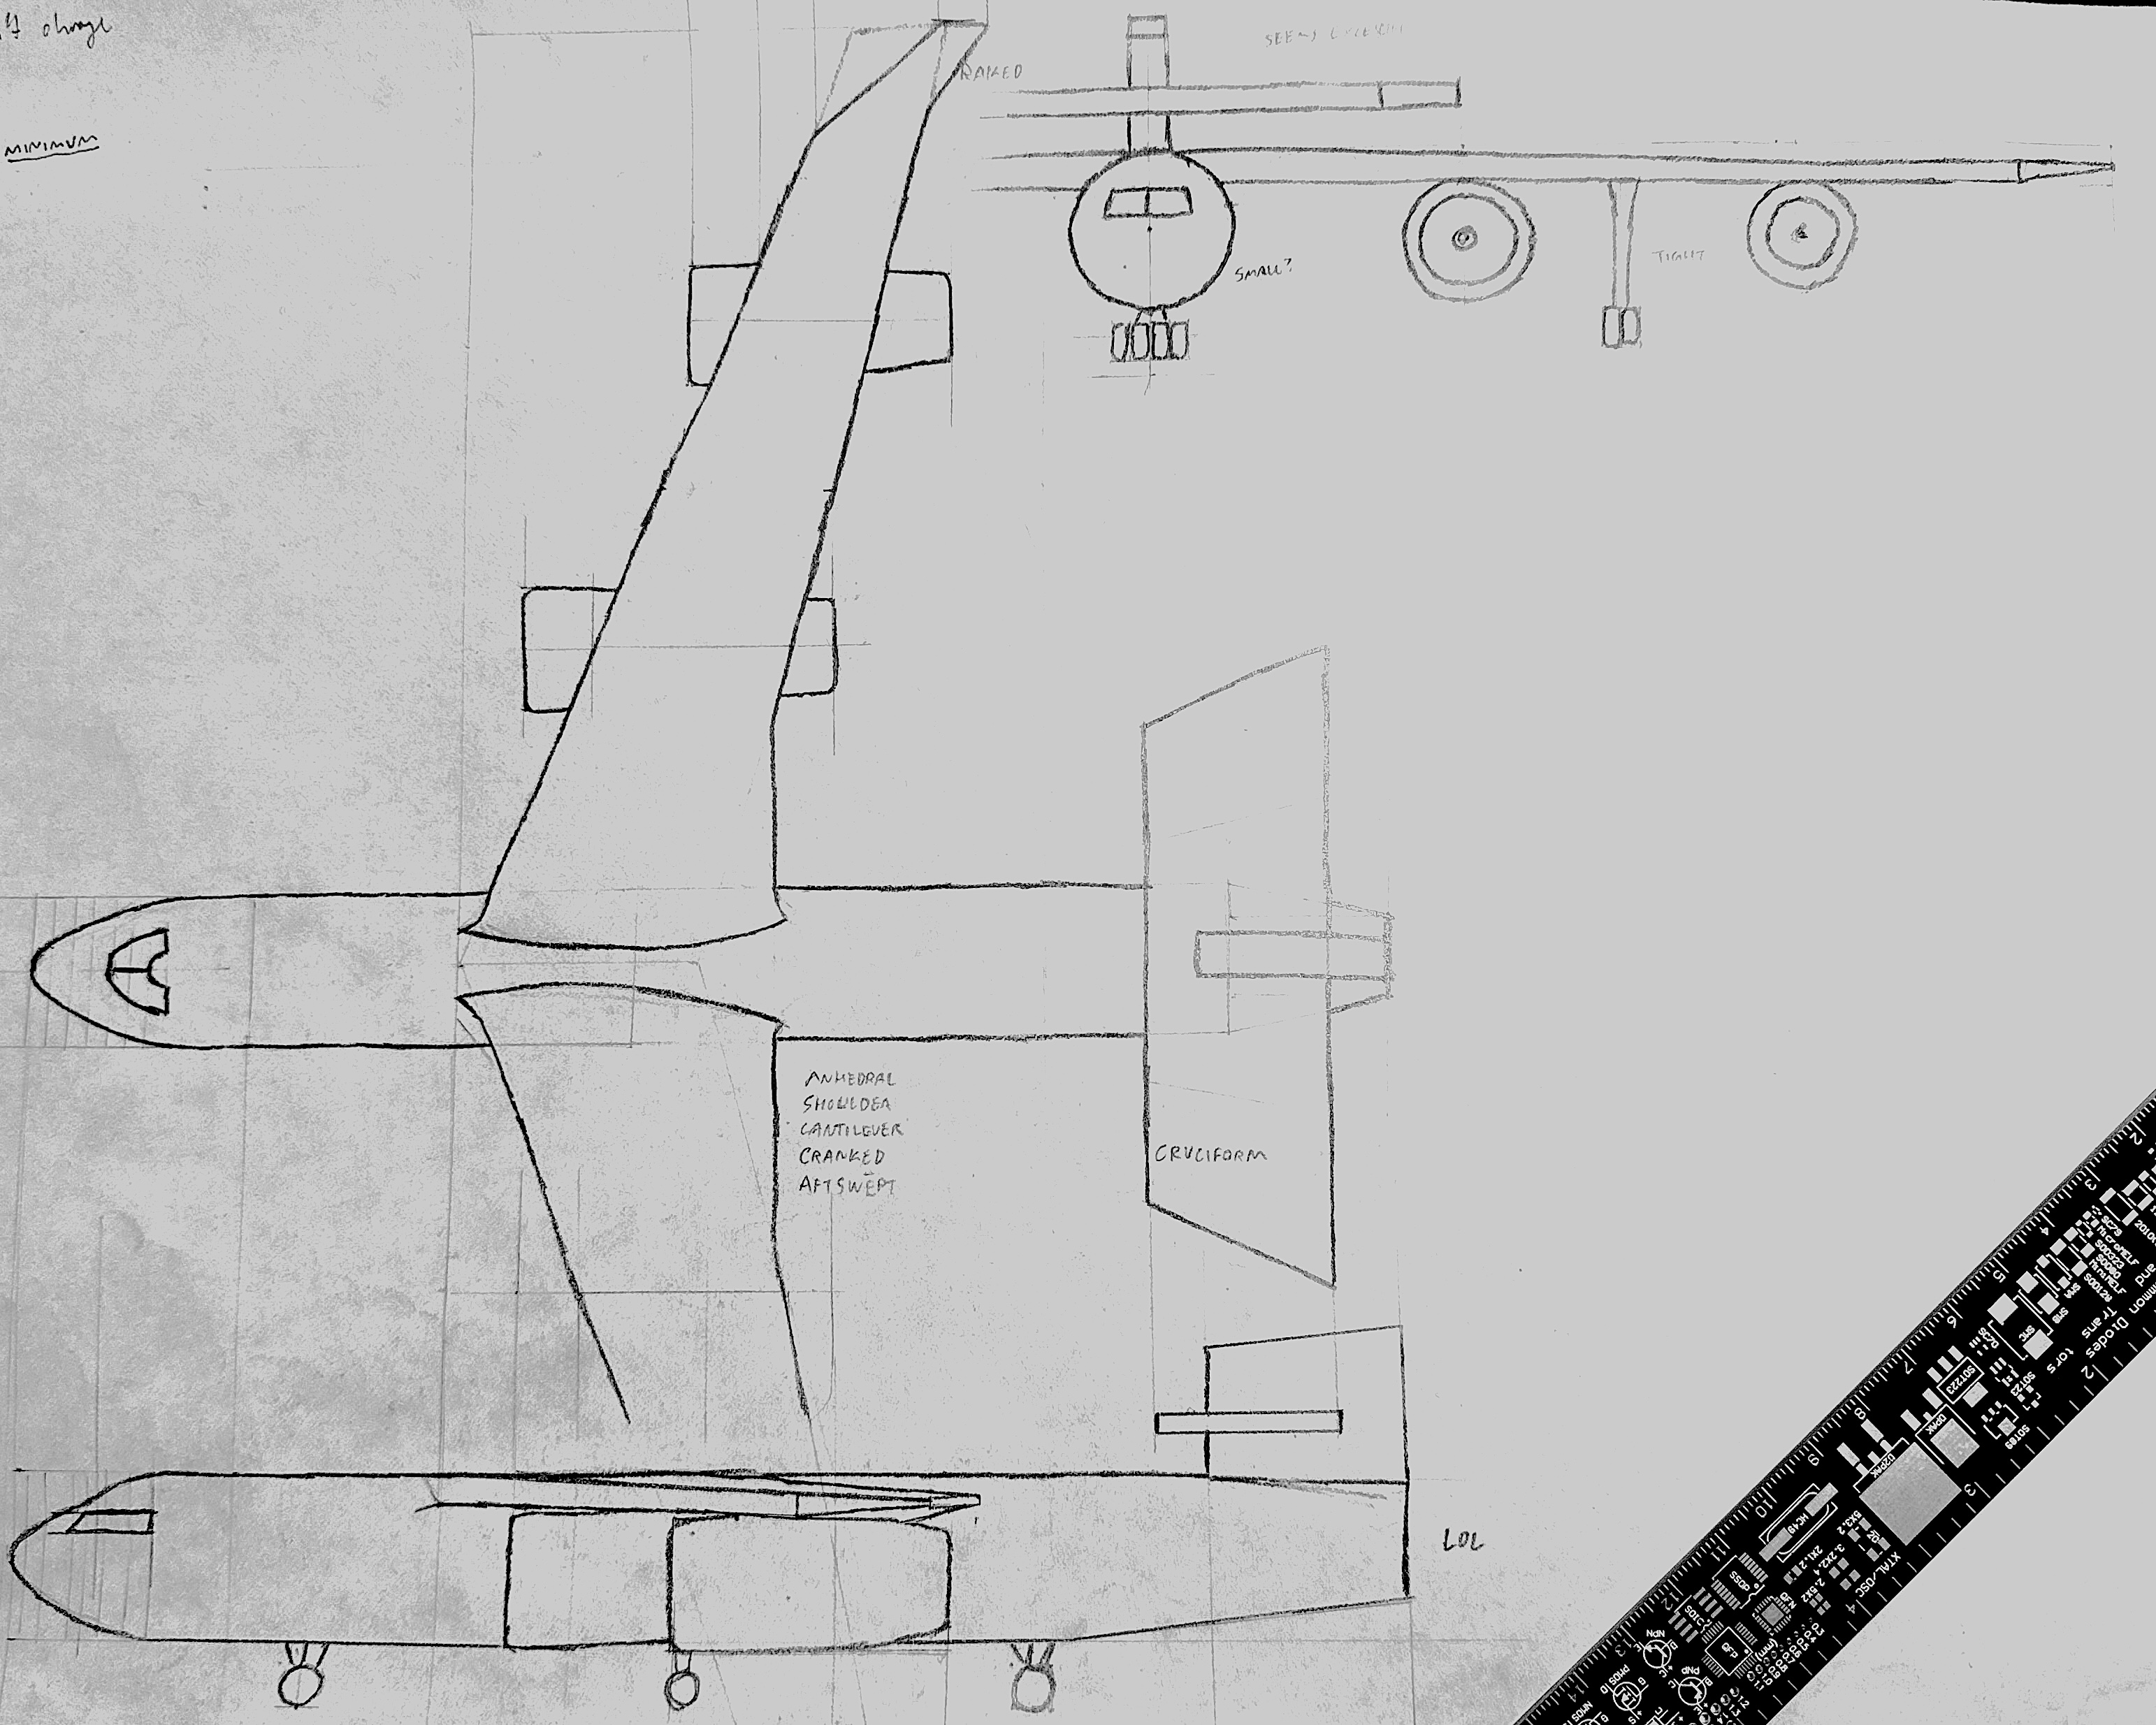
\includegraphics[width=.9\textwidth]{handsketch}
	\caption{Hand-sketched 3-view}
	\label{fig:sketch}
\end{SCfigure}

A hand-sketched 3-view of the STRATODUSTER is presented in Figure~\ref{fig:sketch}.
The general design choices and justifications are laid out in the sections below.
\subsubsection{Fuselage}
\begin{compactenum}
	\item \textbf{Conventional (Tubular) Fuselage} \\ Chosen for its simplicity and versatility.
	\item \textbf{Cargo Door/Ramp} \\ At the rear, the cargo door/ramp will be located for ease of payload access.
	\item \textbf{Cockpit} \\ The crew quarters are located at the front of the fuselage, with a standard roofed cabin.
	\item \textbf{Retractable Tandem Landing Gear with Outriggers} \\ Depending on further analysis, may switch to retractable tricycle.
\setcounter{enumine}{\value{enumi}}
\end{compactenum}

\subsubsection{Wings}
\begin{compactenum}
\setcounter{enumi}{\value{enumine}}
	\item \textbf{Shoulder-wing} \\ Shoulder-wings are chosen for ground clearance and to keep the internals of the fuselage free from interruption.
	\item \textbf{Monoplane} \\ No tangible benefits anticipated from any exotic wing configurations.
	\item \textbf{Anhedral Cantilever} \\ Mainly inspired by the Boeing B-52 and B-47.
	\item \textbf{Cruciform Tail} \\ If the payload is dispensed from anywhere other than the tail (like the wings), want to avoid sulfuric acid spray on tail.
	\item \textbf{Cranked Trapezoidal Planform} \\ The aft sweep is inspired by the Boeing B-52, B-47, and many other high-altitude aircraft, and the cranked geometry is inspired by commercial Boeings and other business jets.
	\item \textbf{Raked Wingtip} \\ Inspired by the Boeing 777 commercial transport aircraft, the Tip A generates the least lift-induced drag of the four wing styles~\cite{textbook}.
\setcounter{enumine}{\value{enumi}}
\end{compactenum}
\subsubsection{Powerplant}
\begin{compactenum}
\setcounter{enumi}{\value{enumine}}
	\item \textbf{Low BPR Turbofan or Turbojet} \\ At the required altitude and crusing speed, props would be ineffective.
	\item \textbf{Quantity} \\ Quantity and configuration (how many engines per pylon) have not been fixed yet.
	\item \textbf{Location} \\ Engines will be located in nacelles on the wings. They can't be located behind the point of payload dispersion, since it's presumably undesirable to have sulfuric acid enter the intakes.
\end{compactenum}

Specific physical dimensions of the aircraft have been intentionally omitted, as there are too many unknowns to fix any dimension yet.
The general form, however, is generally fixed.
Fuselage diameter may change, engine sizes and locations are unknown, wingspan is yet to be determined, along with tail configuration, and the rear of the plane needs work.
Initial airfoil design will be based on the NACA airfoils used in the Boeing B-52 and B-47.
The main driving forces here are that high-altitude aircraft generally need large wings to generate enough lift, and the multi-engine, under-wing configuration is quite standard for many commercial and transport aircraft.
	
	
\section{Cost Analysis}
\subsection{Production Costs}

\subsection{Operation Costs}


\section{Initial Sizing (Weight Analysis)}
\subsection{Design Mission Profile}

\subsection{Preliminary Sizing}

\subsection{Sizing Sensitivity}

\clearpage
\printbibliography[heading=bibnumbered]

\end{document}